\selectlanguage{english}
\begin{abstract}
    \noindent For the second project of the Computer Simulations (ELTE Physics MSc) course I created a molecular dynamics simulation, using the velocity Verlet integration. I also implemented Verlet's pair-list method, along with his Lennard-Jones potential cut-off method. Sadly because of unknown reasons, I could only managed to run the simulation with periodic boundary conditions, instead of both periodic and closed conditions. I also considered the measurement of some thermodynamic quantities, which I did successfully, and compared them with literary data as well. Problems and limits of the simulation are also discussed.
\end{abstract}

\begin{multicols}{2}
\section{Introduction}
In the short description I've already discussed all the details regarding the theoretical background and implemented features. In this document I'll only focus on the discussion of those features, which were actually programmed and tested and won't copy and repeat the whole theoretical and technical details from the short description.

\section{Description of the simulation}
\subsection{Features and functionality}
For the second project I implemented a working molecular dynamics simulation, which intends to simulate the motion of a fairly small number ($N < 1000$) of interacting particles inside a box with periodical boundary conditions at a given $T$ temperature, using the velocity Verlet method. The expected behaviour of simulation was to correctly illustrate the Brownian motion of some interacting particles and the temperature oscillation of its gas around a given temperature. \par
The interaction between the particles are defined with the truncated and shifted Lennard-Jones potential

\begin{equation}
V_{c}^{LJ} \left( r \right)
=
\begin{cases}
4 V_{0} \left[ \left( \frac{\sigma}{r} \right)^{12} - \left( \frac{\sigma}{r} \right)^{6} \right] & \text{if}\ r < r_{c} \\
0 & \text{if}\ r \geq r_{c}
\end{cases}
\end{equation}
Where the \texttt{r\_c} cut-off distance was chosen to be
 
\begin{equation}
\text{\texttt{r\_c}} = 2.5 \sigma
\end{equation}
\begin{center}
	\includegraphics[width=0.45\textwidth]{img_src/{TS_Lennard_Jones_Potential}.pdf}
	\captionof{figure}{The truncated and shifted Lennard-Jones potential} \label{fig:1}
\end{center}
I also implemented Verlet's pair-list method. This means, that I stored the indeces of every particle-pairs, which was situated closer to each other, than a chosen \texttt{r\_max} distance. When the simulation calculates the interaction forces between particles, it only loops over this list, instead of calculating forces between all particles in the simulation. I've chosen a widely used value of this distance to be

\begin{equation}
\text{\texttt{r\_max}} = 3.2 \sigma
\end{equation}
Since the particles moves at a finite speed, it needs some steps, before a non-list element wanders into the interaction sphere of $\text{\texttt{r\_c}} = 2.5 \sigma$. This means we only need to update the pair-list only after some \texttt{update\_interval} number of iterations. I've chosen this number to be
\begin{equation}
\text{\texttt{update\_interval}} = 10
\end{equation}
To regularize the system, I've rescaled the velocities at every $200$th step, to ensure the simulation never blows up. \par
Besides these mentioned values, I've used the following constants for my simulation to create the graphs in this report:
\begin{center}
\begin{tabular}{|c|c|}
\hline
Quantity                  & Value \\ \hline \hline
Particle number (N)       & 64    \\ \hline
Temperature (T)           & 50 K  \\ \hline
Step size (dt)            & 0.001 \\ \hline
Particle density ($\rho$) & 1.2   \\ \hline
\end{tabular}
\end{center}
The particle density $\rho$ was used to distribute the particles evenly in a box (discussed in Sec. V.)

\subsection{Used measure}
To choose correct initial velocities, I've used two type of methods. One, the \texttt{gasdev()} function from the \emph{Numerical Recipes} book \citep{press2007numerical} which I've already mentioned in the short description and which I've used last semester, when tried to replicate a molecular dynamics simulation in \texttt{C++} and two, a built-in function in Python's NumPy library, named \texttt{numpy.random.normal()}. Both of them generates normally distributed random numbers, with $\sigma = 1$ value.

\begin{center}
    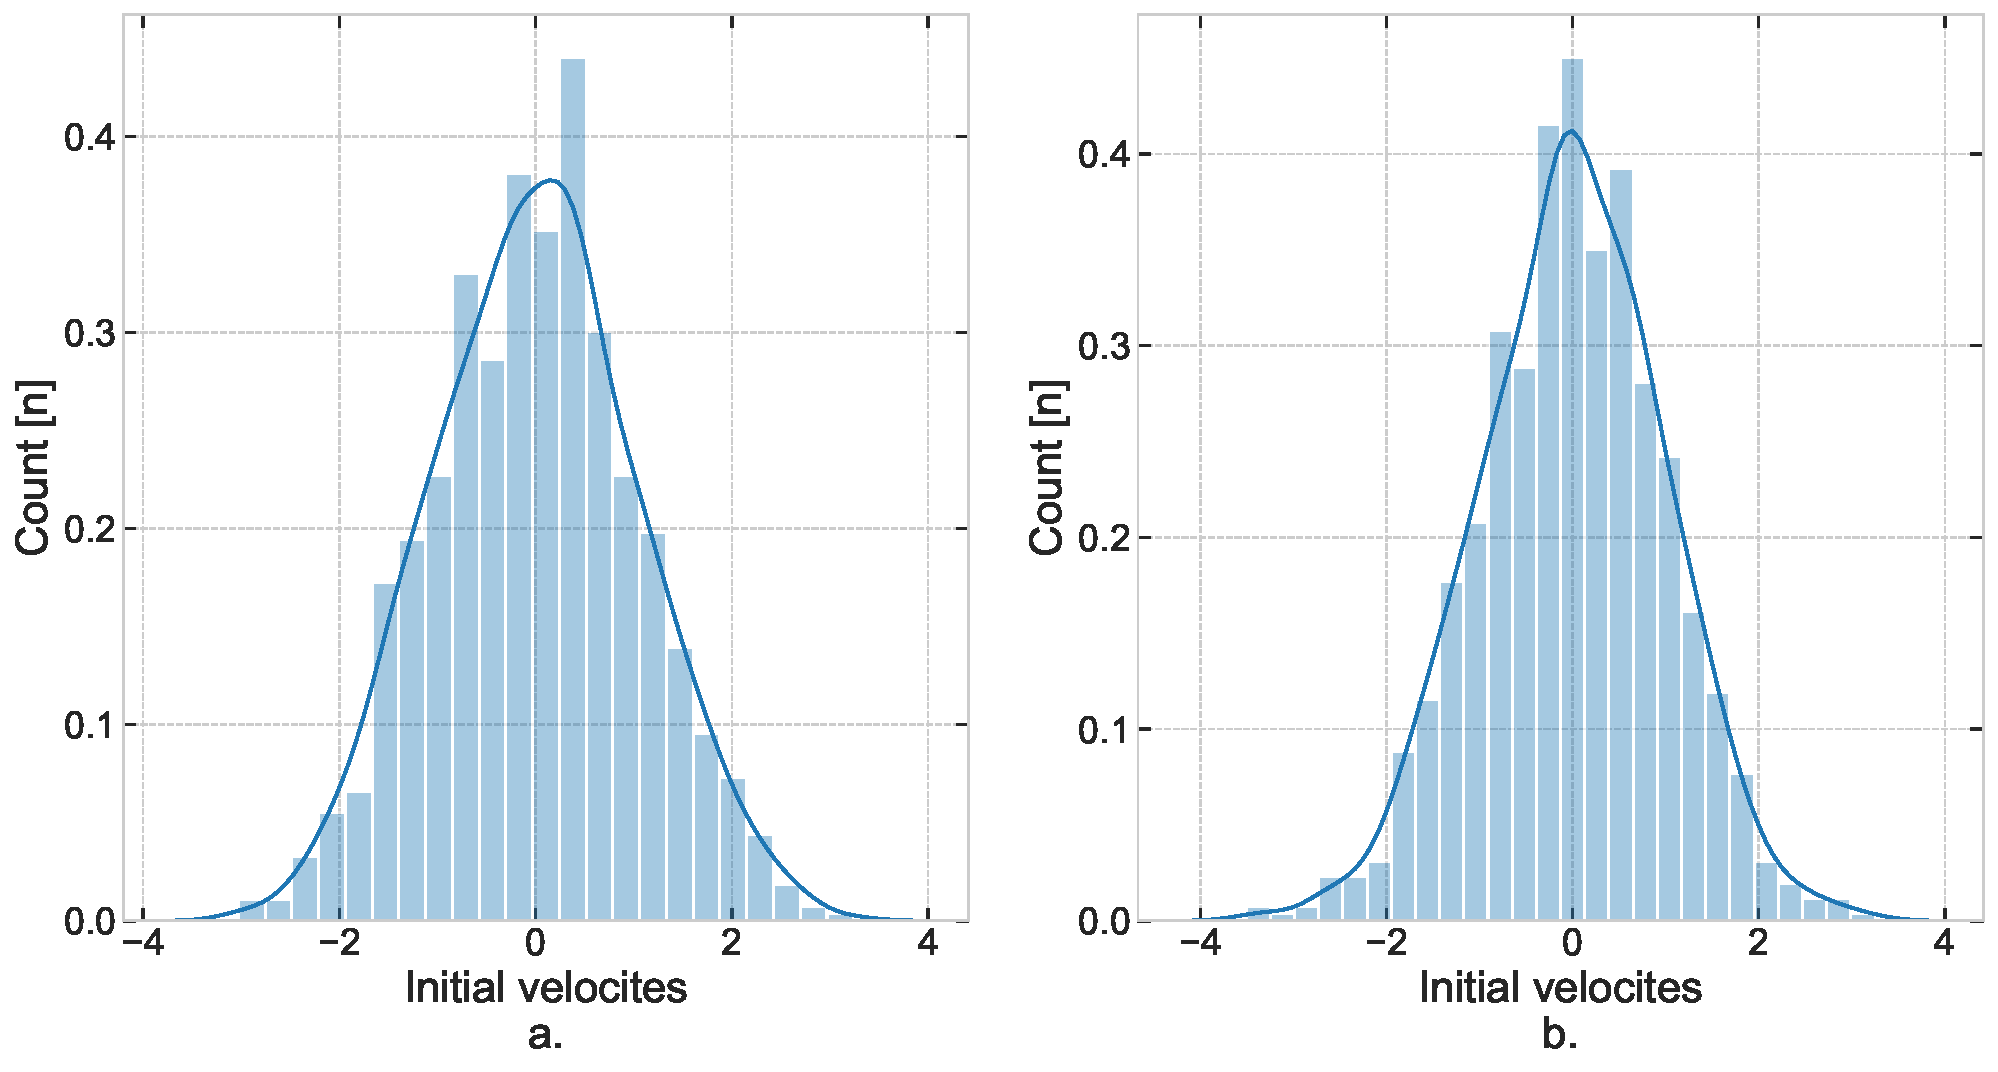
\includegraphics[width=0.45\textwidth]{{img_src/compare_velocity_distribution}.pdf}
    \captionof{figure}{Comparing the Box-Müller algorithm with NumPy's built-in \texttt{numpy.random.normal()} function.\\a. Box-Müller algorithm\\b. NumPy's \texttt{numpy.random.normal()}} \label{fig:2}
\end{center}
Running the simulation with either models, did not seem to make any difference, since both of their outputs are corrected with the already discussed transformation in the short description. \par
Physically, the velocity distribution of particles in a gas could be described by the discussed Gauss distribution:

\begin{equation}
P \left( v \right)
=
\left( \frac{m}{2 \pi k_{B} T} \right)^{3/2}
*
e^{-\dfrac{m \left( v_{x}^{2} + v_{y}^{2} + v_{z}^{2} \right)}{2 k_{B} T}}
\end{equation}
However, the two mentioned methods generates such velocity values, which correspond to the measure
\begin{equation}
k_{B} = N_{A} = \sigma = m = T = 1.
\end{equation}
To make the calculations consistent, I've used this measure throughout everywhere in the simulation, except the $T = 1$ condition. Where the velocities are rescaled by a $\lambda$ constant

\begin{equation}
\lambda
=
\sqrt{\frac{2 \left( N - 1 \right) k_{B} T}{\sum_{i=1}^{N} m \boldsymbol{v}_{i}^{2}}}
\end{equation}
I've used the following form for this constant:
\begin{equation}
\lambda
=
\sqrt{\frac{2 \left( N - 1 \right) T}{\sum_{i=1}^{N} \boldsymbol{v}_{i}^{2}}}
\end{equation}
where $T$ is the temperature and could be freely given at the start of the simulation, despite the fact, that either at the \texttt{gasdev()} or \texttt{numpy.random.normal()} step we ignore its value. However this does not affect the simulation in such way, which we should deeper investigate in this course.

\begin{center}
    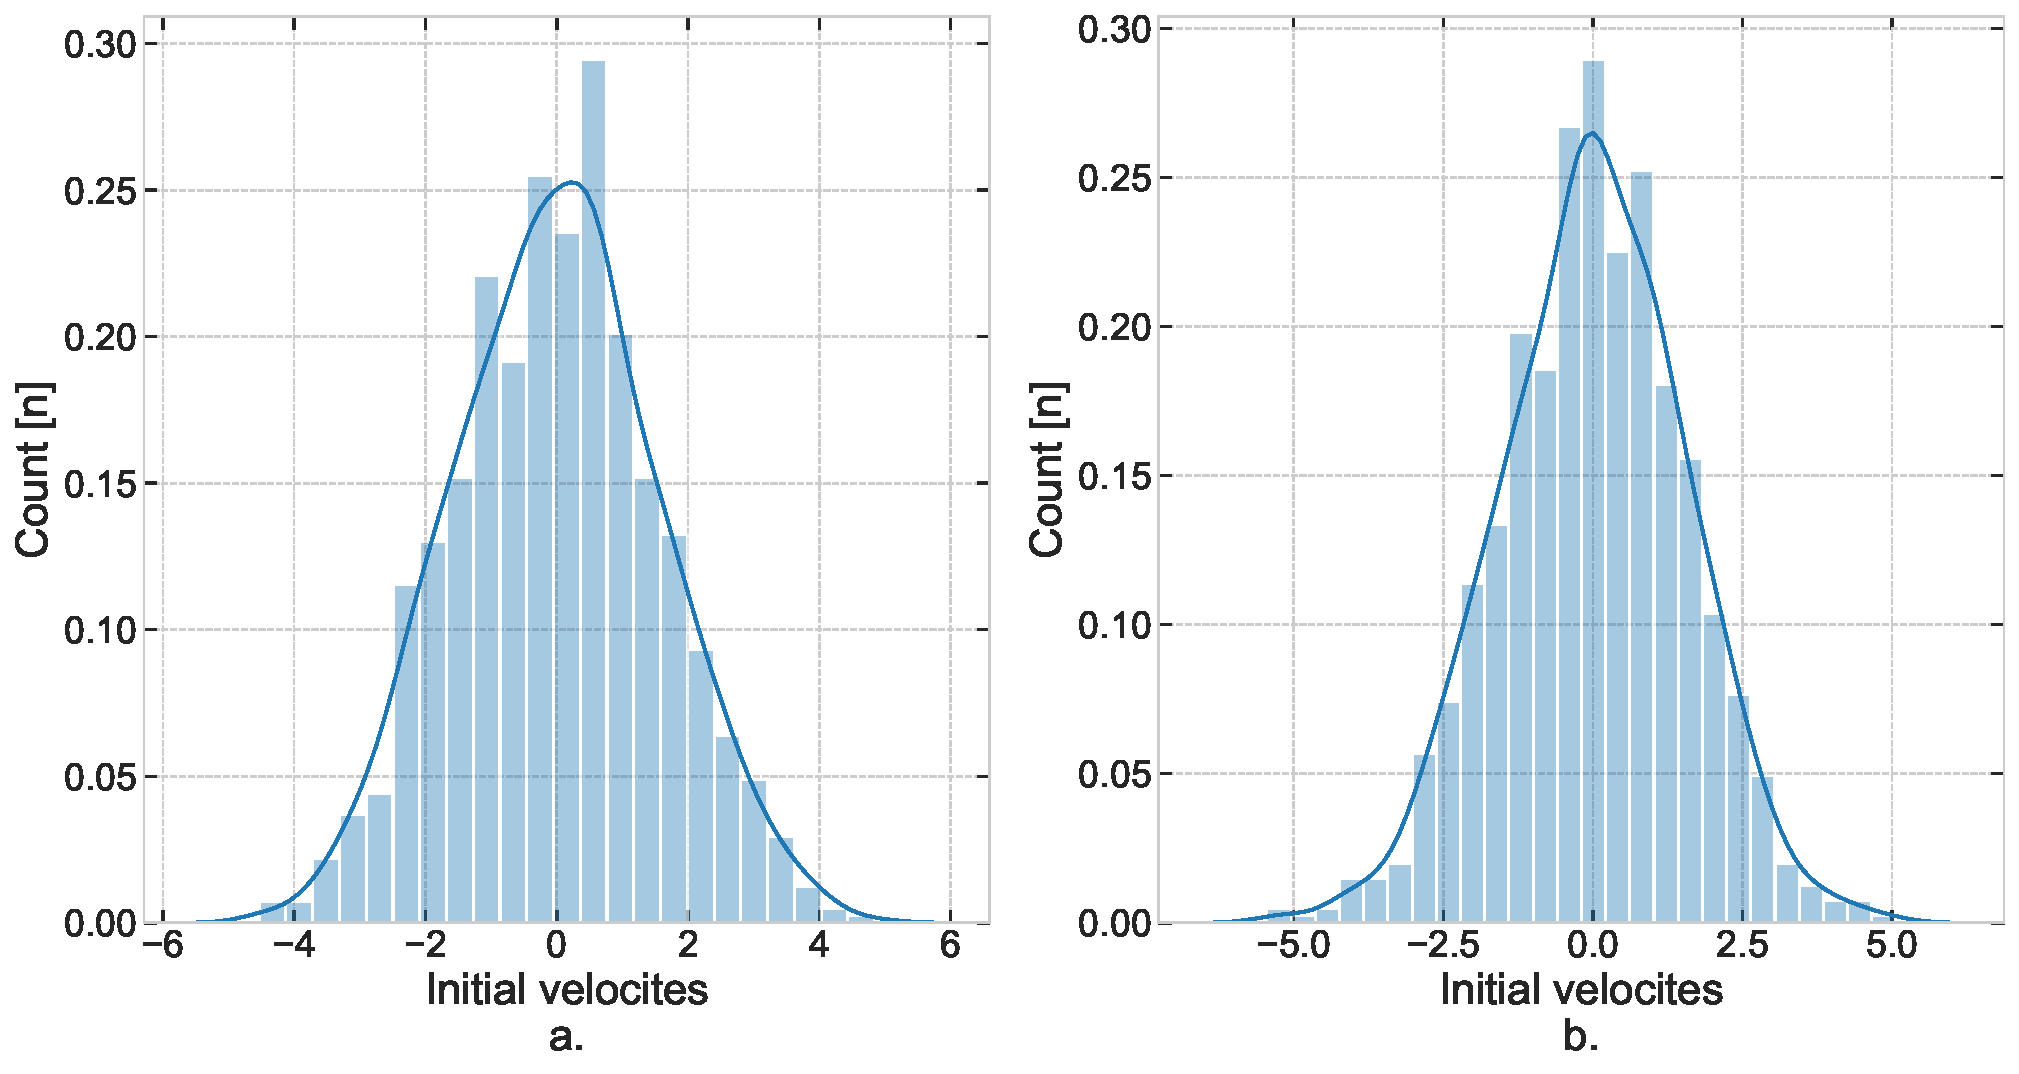
\includegraphics[width=0.45\textwidth]{{img_src/compare_transformed_velocity_distribution}.pdf}
    \captionof{figure}{Comparing the distribution of the transformed and rescaled velocities for $T = 1$, initially generated by the Box-Müller algorithm and NumPy's built-in \texttt{numpy.random.normal()} function.\\a. Box-Müller algorithm\\b. NumPy's \texttt{numpy.random.normal()}} \label{fig:3}
\end{center}

\section{Direct results}
The model was proved to be considerably robust in a way, that it always gave physically meaningful results. During runtime in every step I've measured the values of numerous quantities. I plotted the changing of the values which could be seen from Fig. (\ref{fig:4}) - Fig. (\ref{fig:8}). These measured values were the following: \\
1. Kinetic energy:
\begin{equation}
K
=
\frac{1}{2} \sum_{i} m_{i} * \boldsymbol{v}_{i}^{2}
=
\frac{1}{2} \sum_{i} \boldsymbol{v}_{i}^{2}
\end{equation}
\begin{center}
    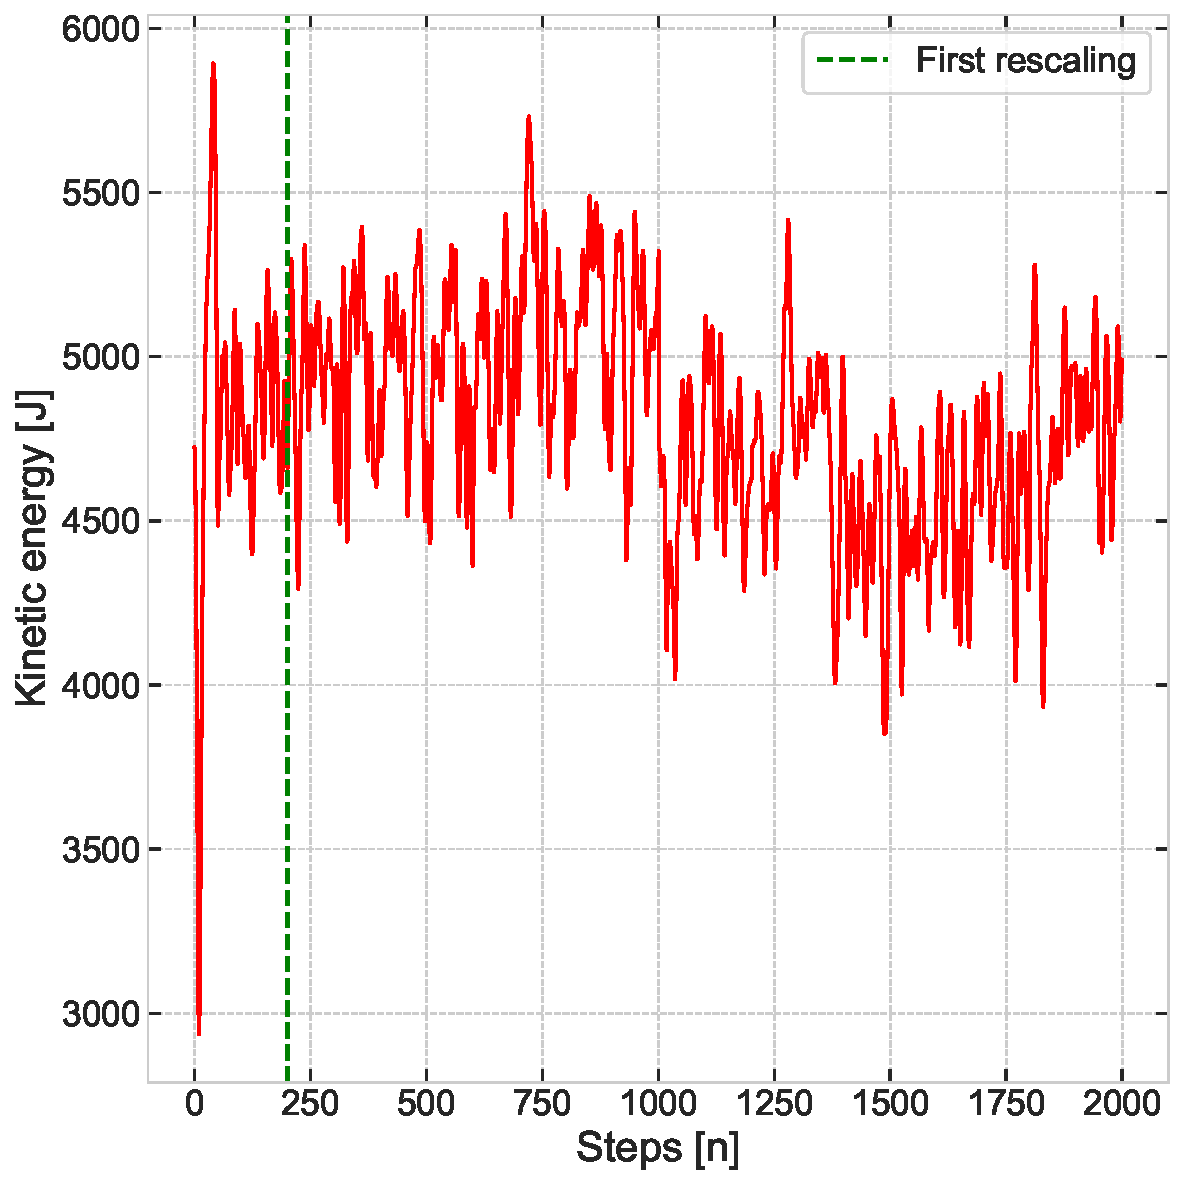
\includegraphics[width=0.45\textwidth]{{img_src/instantaneous_kinetic_E_2000}.pdf}
    \captionof{figure}{Kinetic energy change of the system with 64 particles for $2000$ steps with dt$= 0.001$ step size.} \label{fig:4}
\end{center}
2. Potential energy:
\begin{equation}
V
=
\sum_{i} 4 * V_{0}
*
\left[
\left( \frac{\sigma}{\left| \boldsymbol{r}_{i} - \boldsymbol{r}_{j} \right|} \right)^{12}
-
\left( \frac{\sigma}{\left| \boldsymbol{r}_{i} - \boldsymbol{r}_{j} \right|} \right)^{6}
\right]
\end{equation}
\begin{center}
    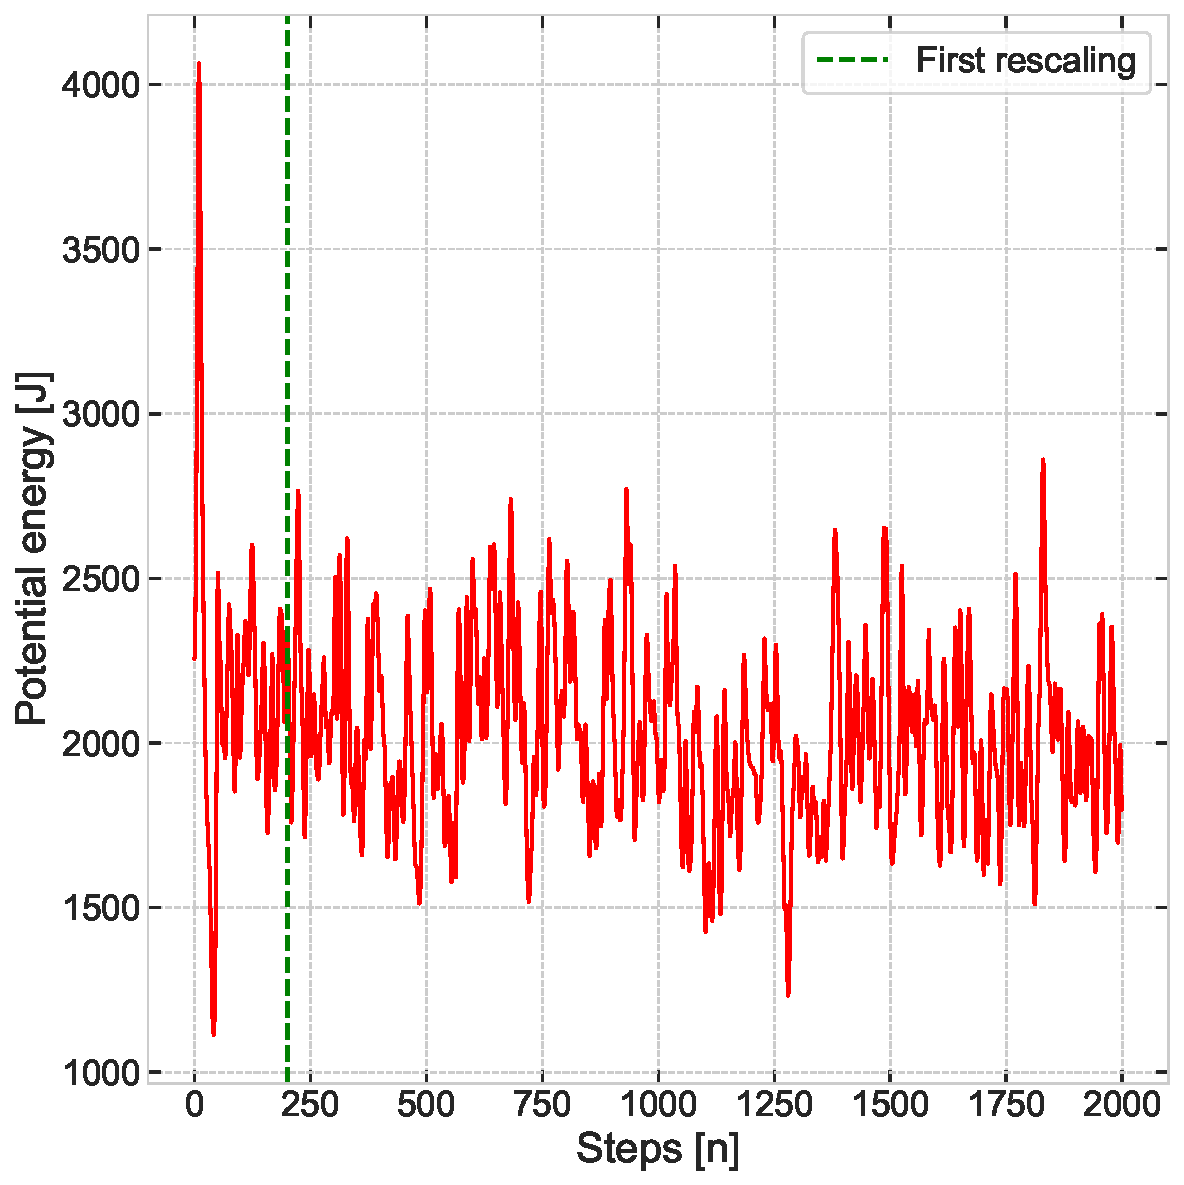
\includegraphics[width=0.45\textwidth]{{img_src/instantaneous_potential_E_2000}.pdf}
    \captionof{figure}{Potential energy change of the system with 64 particles for $2000$ steps with dt$= 0.001$ step size.} \label{fig:5}
\end{center}
3. Total energy, which is simply
\begin{equation}
H
=
K + V
\end{equation}
\begin{center}
    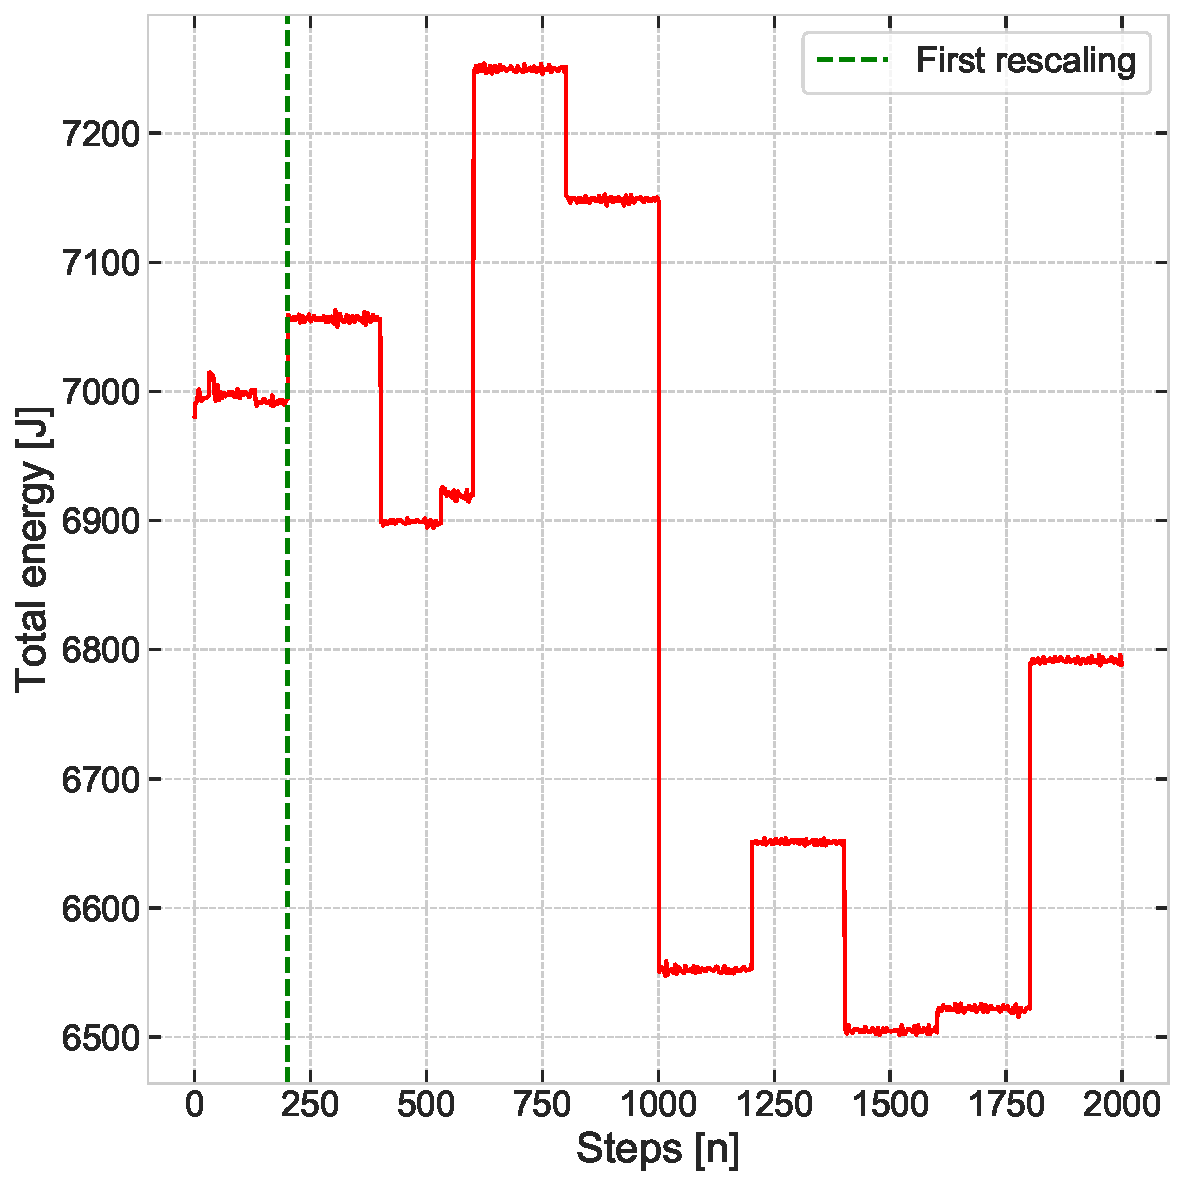
\includegraphics[width=0.45\textwidth]{{img_src/instantaneous_total_E_2000}.pdf}
    \captionof{figure}{Total energy (K + V) of the system with 64 particles for $2000$ steps with dt$= 0.001$ step size.} \label{fig:6}
\end{center}
This quantity should be always constant. It could be well seen on Fig. (\ref{fig:6}), that energy remains totally stable and constant during the run, and only changes its value instantaneously, when the velocities are rescaled after every $200$th step to regularize the system. \\
4. Energy dimensional quantity in Virial theorem, needed for the calculation of the system's pressure:
\begin{equation}
\sum_{i\ <\ j} \boldsymbol{r}_{i} \boldsymbol{F}_{ij}
\end{equation}

Where the values of $F_{ij}$ was already discussed in the short description:
\begin{equation}
\boldsymbol{F} \left( r \right)
=
-\boldsymbol{\nabla} V^{LJ} \left( r \right)
=
\frac{24 V_{0}}{r^{2}} \left[ 2 \left( \frac{\sigma}{r} \right)^{12} - \left( \frac{\sigma}{r} \right)^{6} \right] \boldsymbol{r}
\end{equation}
\begin{center}
    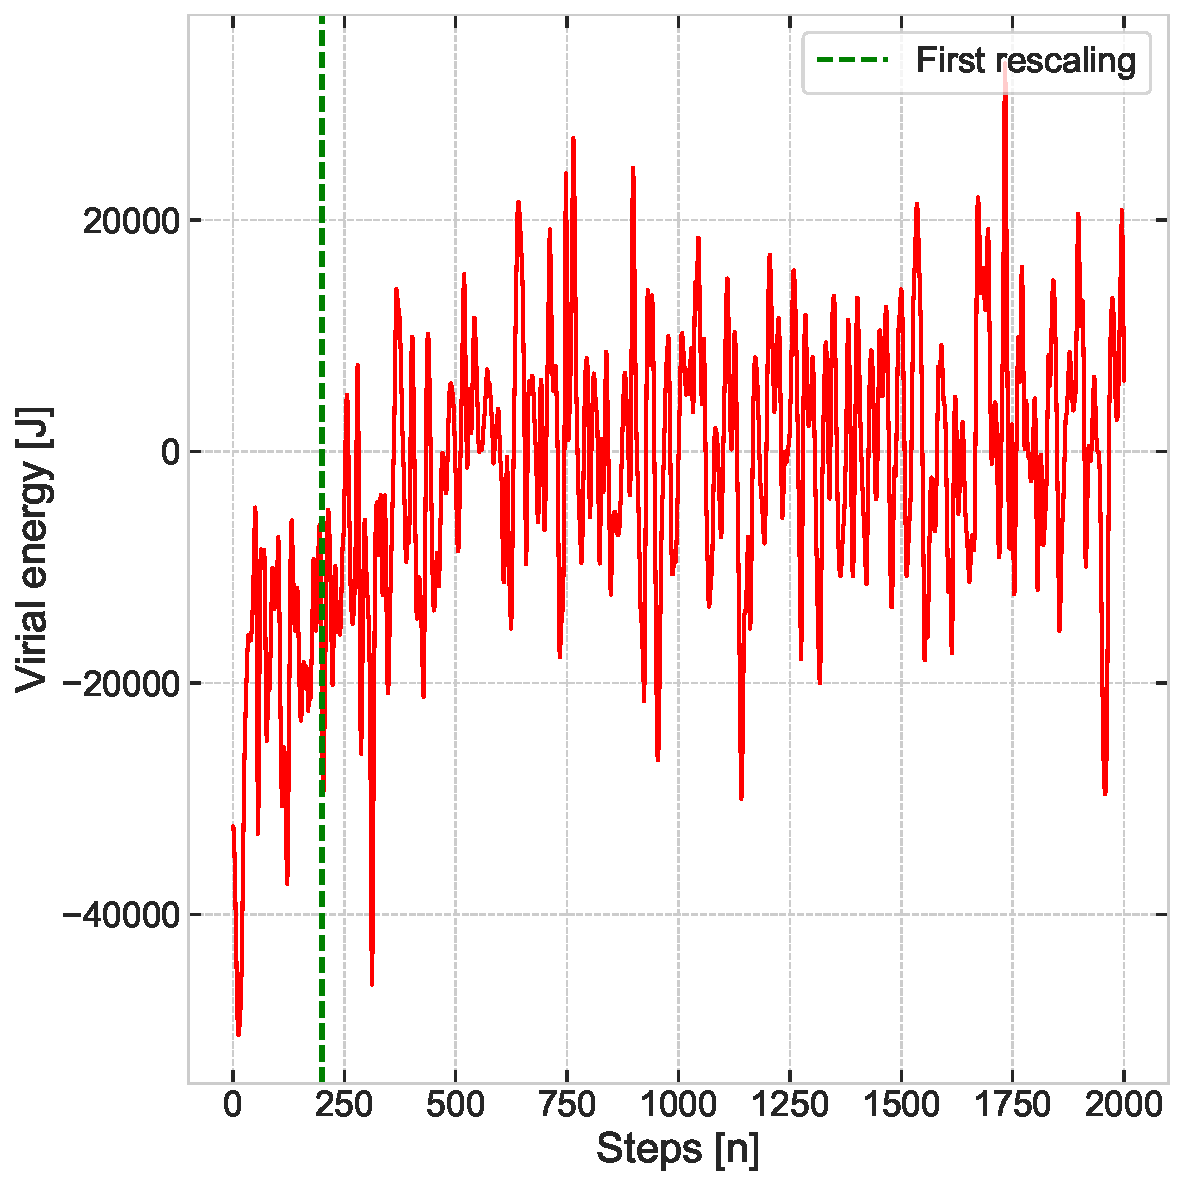
\includegraphics[width=0.45\textwidth]{{img_src/instantaneous_virial_E_2000}.pdf}
    \captionof{figure}{"Virial energy" change of the system with 64 particles for $2000$ steps with dt$= 0.001$ step size.} \label{fig:7}
\end{center}
5. And lastly, the instantaneous temperature of the system:
\begin{equation}
T
=
\frac{\sum_{i} m_{i} * \boldsymbol{v}_{i}^{2}}{3 * \left( N - 1 \right)}
=
\frac{\sum_{i} \boldsymbol{v}_{i}^{2}}{3 * \left( N - 1 \right)}
\end{equation}
\begin{center}
    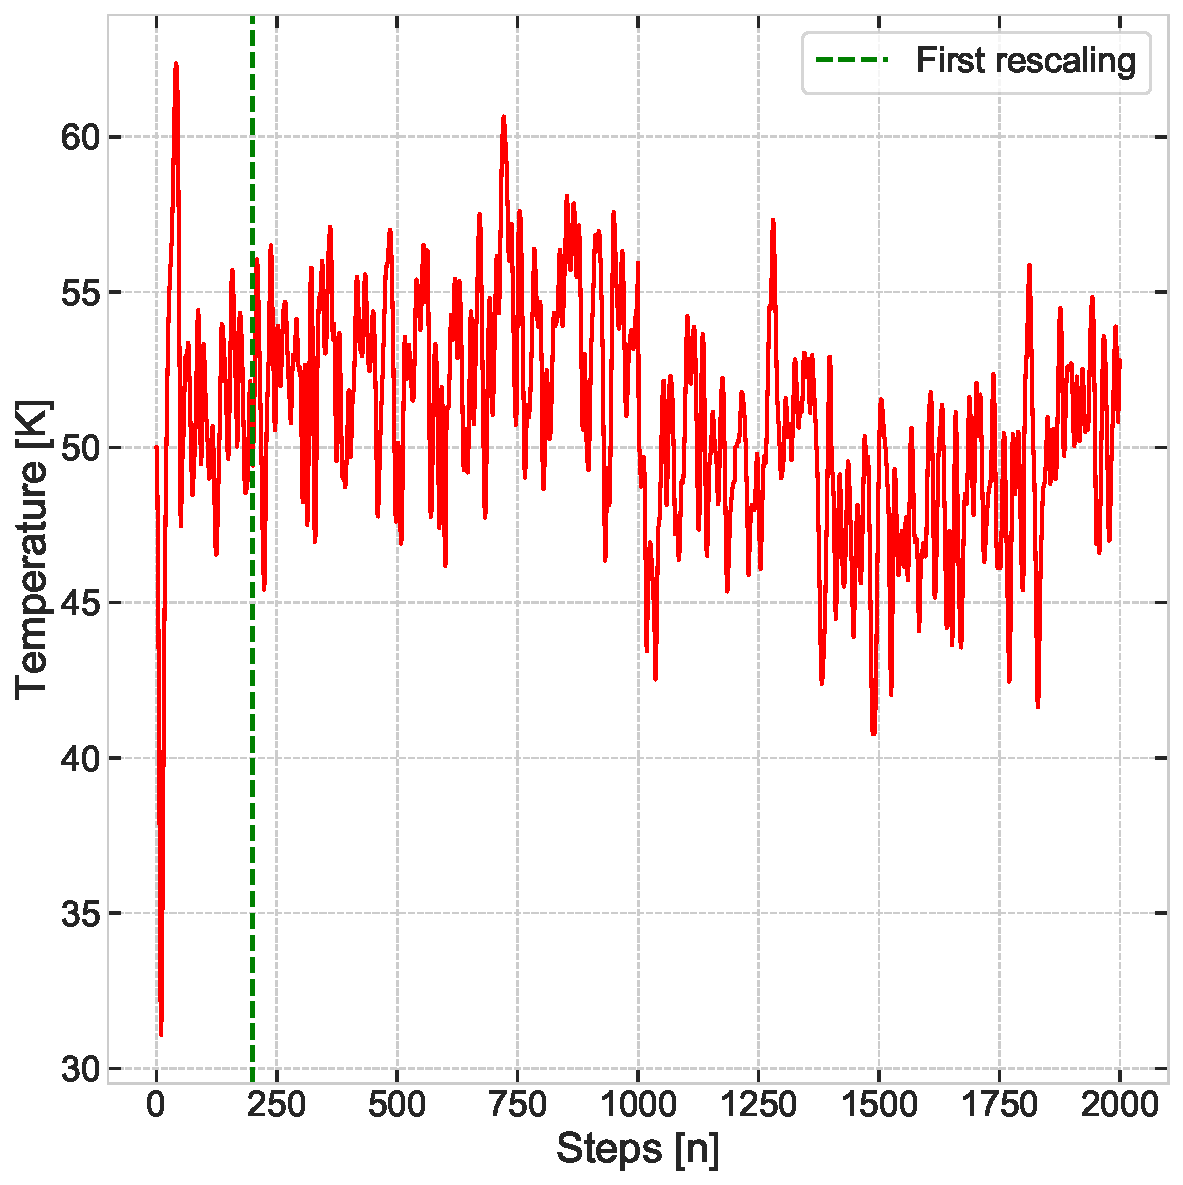
\includegraphics[width=0.45\textwidth]{{img_src/instantaneous_temperatures_2000}.pdf}
    \captionof{figure}{Temperature change of the system with 64 particles for $2000$ steps with dt$= 0.001$ step size.} \label{fig:8}
\end{center}
I did also tracked the coordinate-, velocity- and acceleration changes of the individual particles, and made a nice visualization, which should be helpful to understand the behaviour of the system. For $2\,000$ and $20\,000$ steps I plotted the Brownian oscillation and motion of the system's particles, which could be seen on Fig. (\ref{fig:traj_2000}) and Fig. (\ref{fig:traj_20000}). For a more pleasurable visual experience, some animations could be seen on my YouTube channel\footnote{Link to my YouTube channel: \url{https://www.youtube.com/channel/UCBDSB7PdQ3E9l9WSBsTy7cQ}} inside my "Molecular Dynamics" playlist. Unfortunately these animations were made by me last semester, and thus they don't exactly represent my current results, since I've changed the used code and method a lot since then. However I still wanted to mention them, because they could be still very helpful to understand, what is really happening in this simulation.

\section{Measured thermodynamic quantities}
Using the direct results and data from the simulation I could approximate the values of some thermodynamic quantities also. This goal was attempted by me last semester, but all I've got was totally bad, and meaningless results. Fortunately this semester I've succeeded to calculate some of these quantities and compare them to literary data as well and it was a pretty good match. Namely, these quantities were the molar heat capacity, the pressure and the compressibility factor of the system. To get more robust and accurate results, I've kept the simulation running for $60\,000$ steps to let values which are approximated by their average over time to converge. The first quantity which I've measured was the variance of the total energy:
\begin{equation*}
\left[
\left< E^{2} \right> - \left< E \right>^{2}
\right]
\end{equation*}
To make this quantity converge, I've monitored the changes of the $\left< E \right>$ and $\left< E^{2} \right>$ expected values. When I've seen, they've converged without a doubt, I stopped the simulation. It was at $\approx 60\,000$ steps.
\begin{center}
    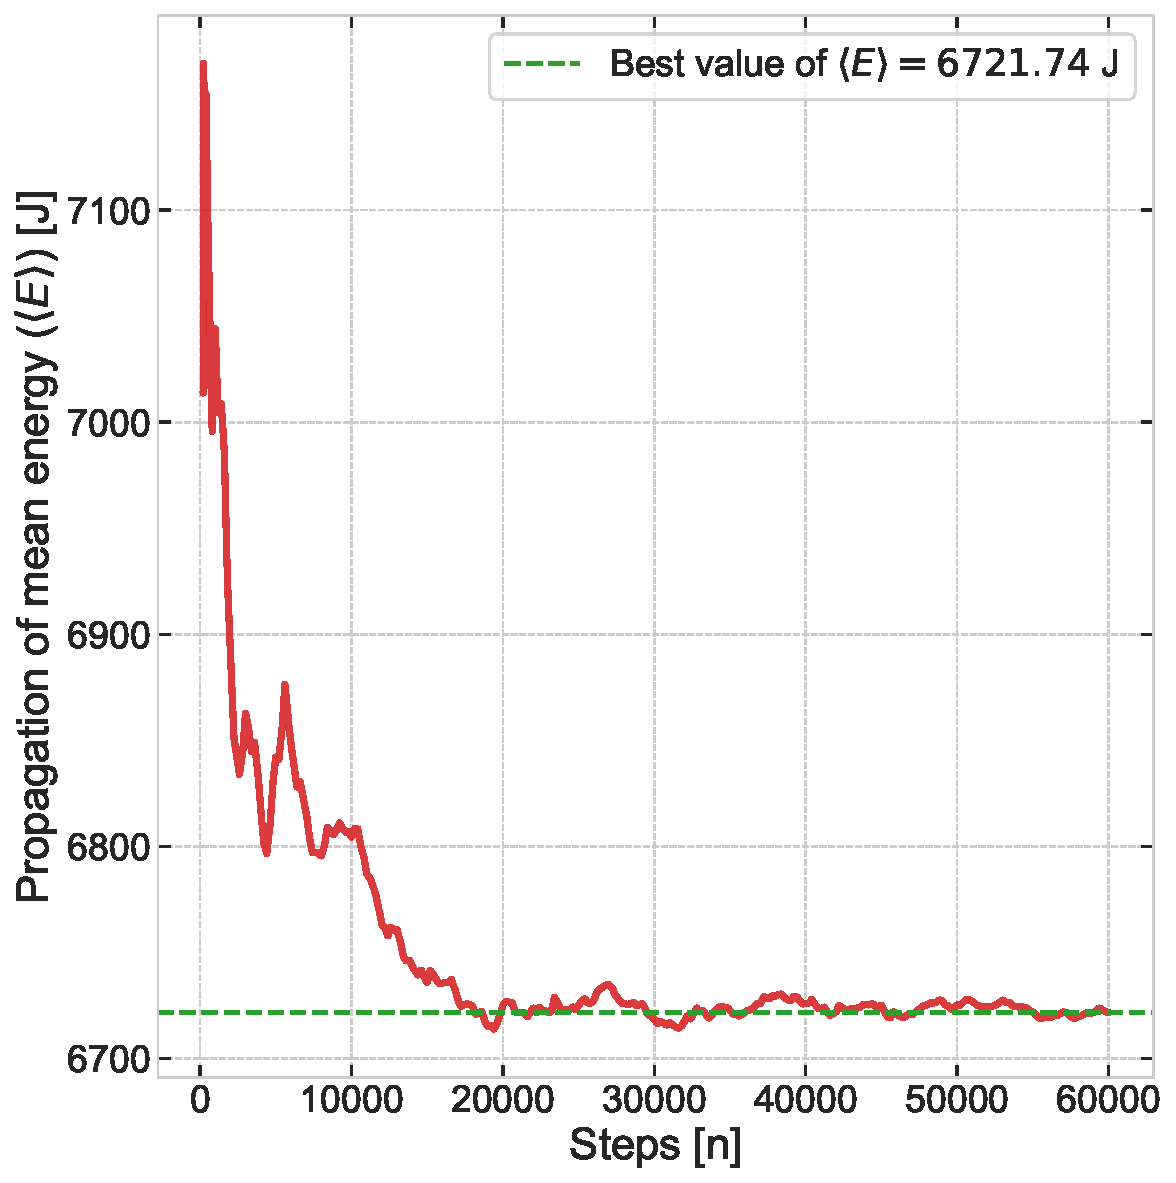
\includegraphics[width=0.45\textwidth]{{img_src/energy_propagation_60000}.pdf}
    \captionof{figure}{Expected value of total energy of the system with 64 particles for $60000$ steps with dt$= 0.001$ step size.} \label{fig:9}
\end{center}
\begin{center}
    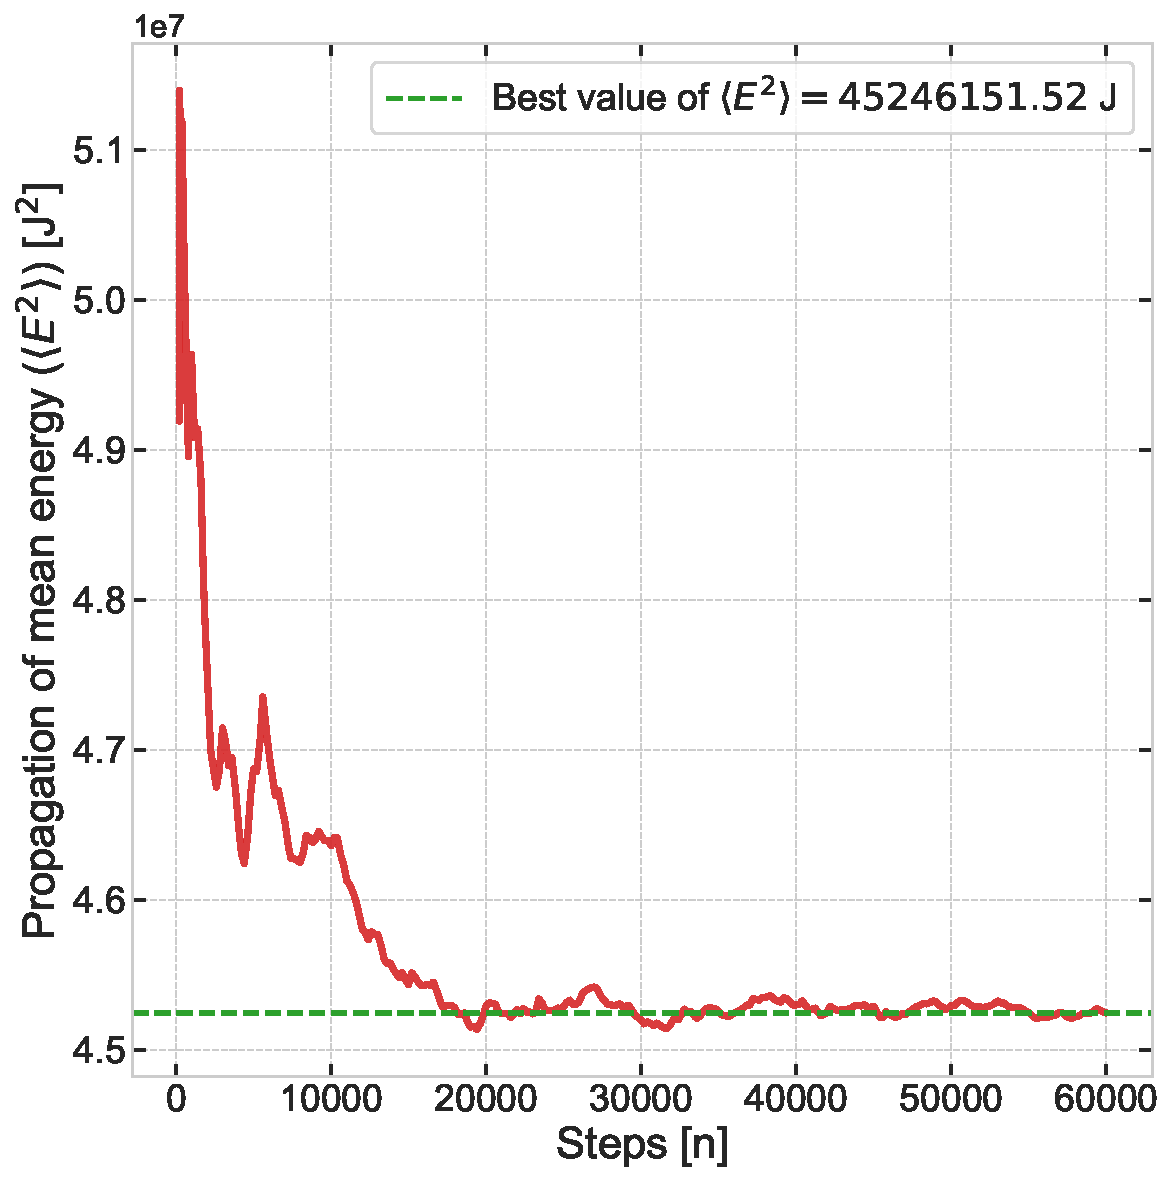
\includegraphics[width=0.45\textwidth]{{img_src/energy_squared_propagation_60000}.pdf}
    \captionof{figure}{Expected value of squared total energy of the system with 64 particles for $60000$ steps with dt$= 0.001$ step size.} \label{fig:10}
\end{center}
Using these quantities I've successfully measured an approximate value for the variance of the total energy.
\begin{center}
    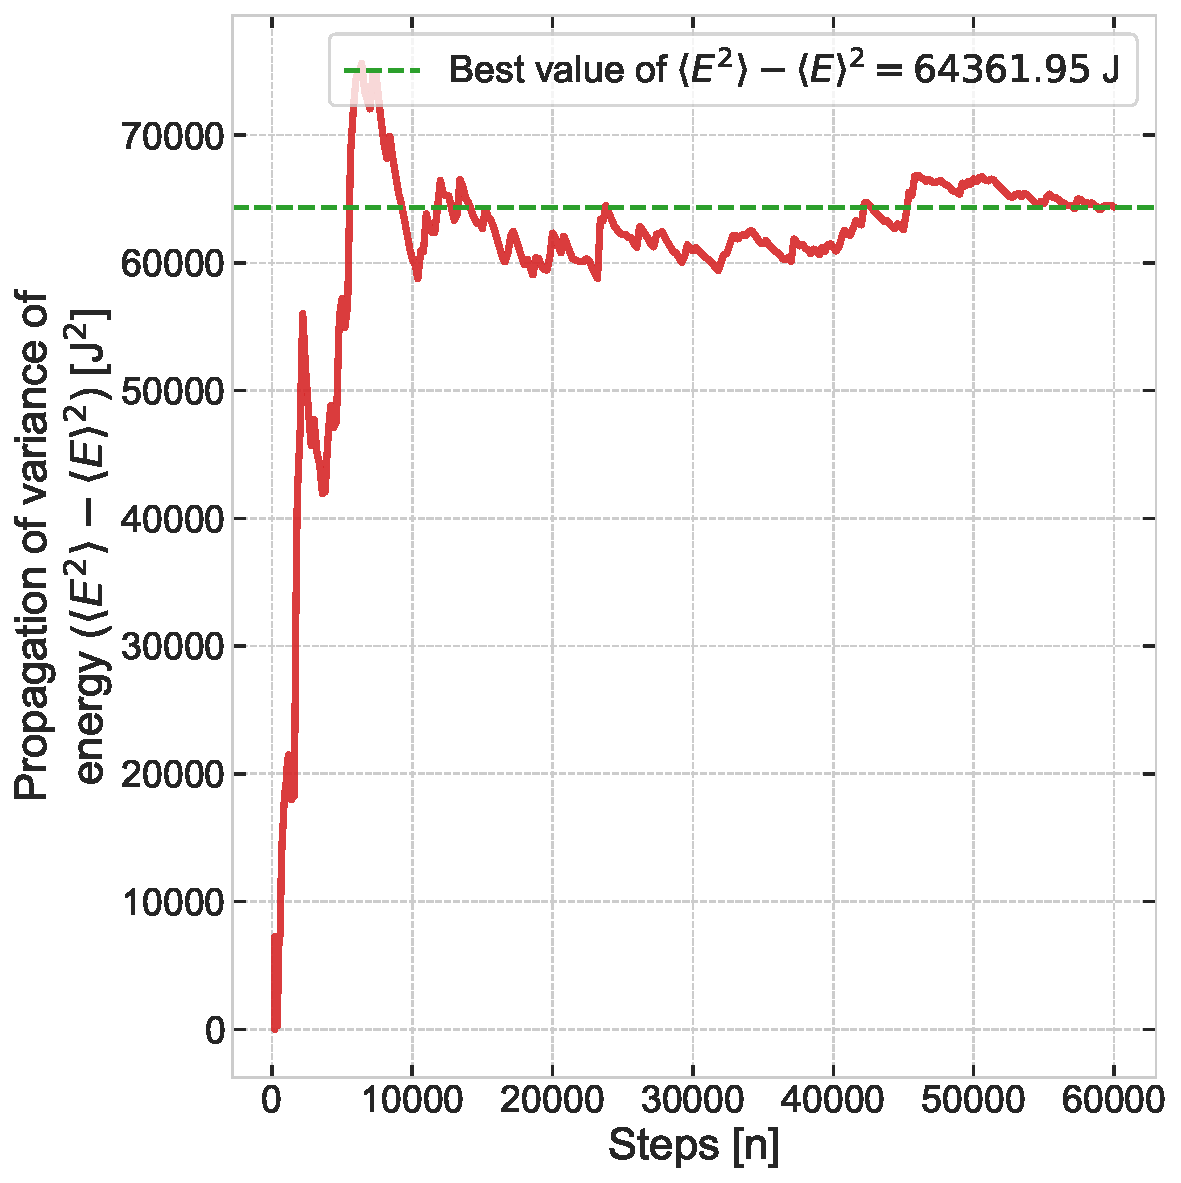
\includegraphics[width=0.45\textwidth]{{img_src/energy_variance_propagation_60000}.pdf}
    \captionof{figure}{Change in the variance of energy of the system with 64 particles for $60000$ steps with dt$= 0.001$ step size.} \label{fig:11}
\end{center}
First, the molar heat capacity was calculated, which definition as discussed in the short description:

\begin{equation}
C_{V}
=
\left. \frac{\partial E}{\partial T} \right|_{V}
=
\frac{1}{k_{B} T^{2}} \left[ \left< E^{2} \right> - \left< E \right>^{2} \right]
\end{equation}
Which in our measure is the following:
\begin{equation}
C_{V}
=
\frac{1}{T^{2}} \left[ \left< E^{2} \right> - \left< E \right>^{2} \right]
\end{equation}
Using the instantaneous temperature values as $T$ and the variance values seen on Fig. (\ref{fig:11}), a propagating value for $C_{V}$ could be plotted, which could be seen on Fig. (\ref{fig:12}).
\begin{center}
    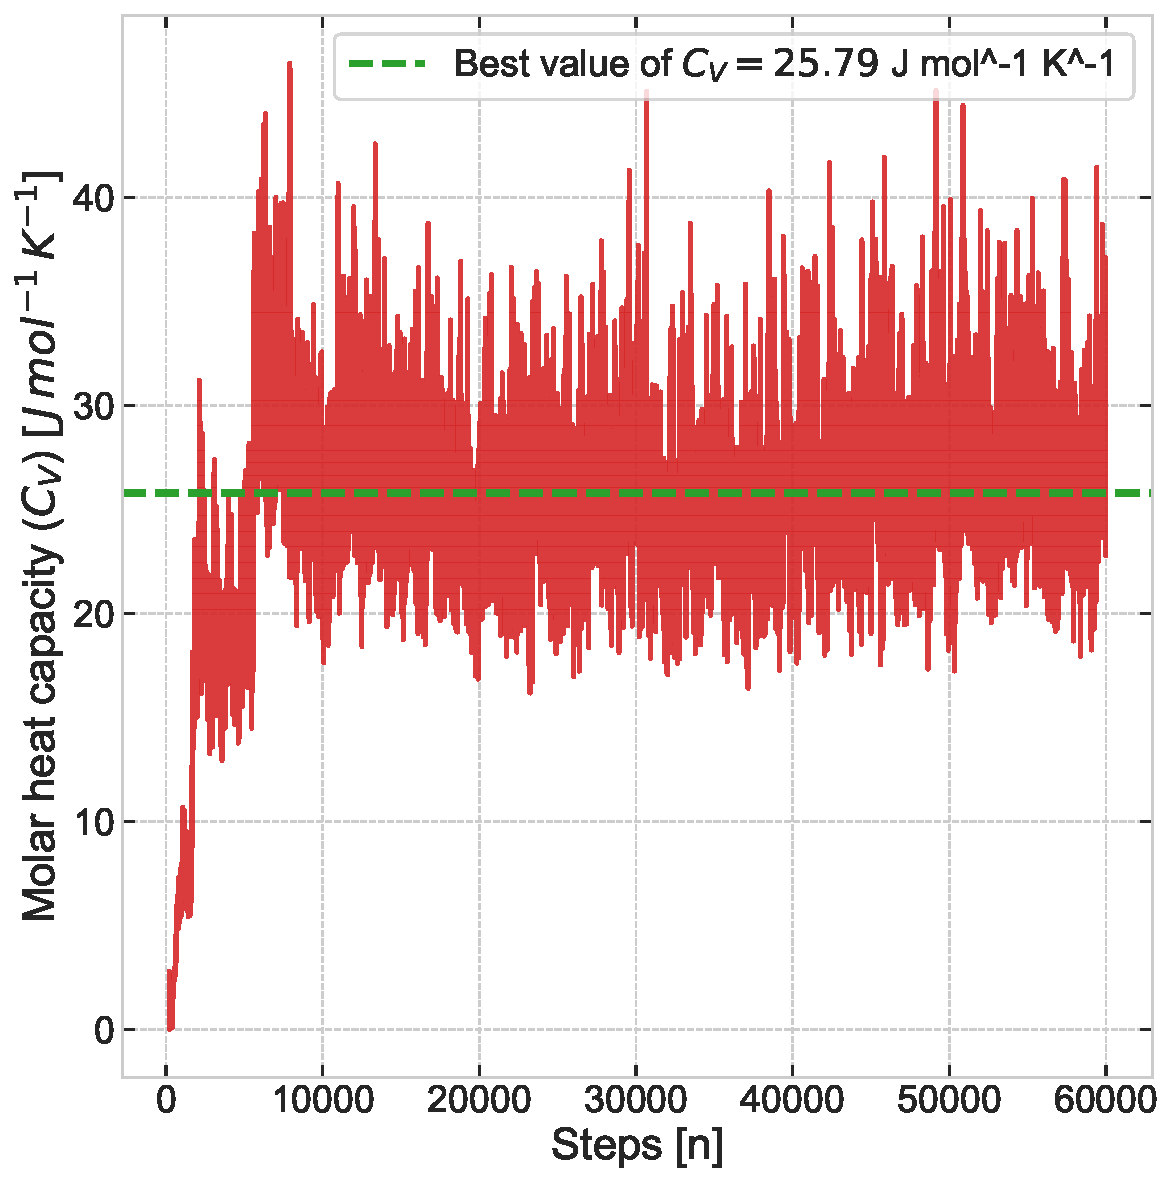
\includegraphics[width=0.45\textwidth]{{img_src/C_V_propagation_60000}.pdf}
    \captionof{figure}{Molar heat capacity on constant volume of the system with 64 particles for $60000$ steps with dt$= 0.001$ step size.} \label{fig:12}
\end{center}
When using the best value for the variance of energy and the mean of the instantaneous temperatures as a value for $T$, then an exact/mean value could be given, which my best result for the $C_{V}$:

\begin{equation}
C_{V}
\approx
25.79\ \frac{\text{J}}{\text{mol K}}
\end{equation}
In literary data, this value for simple gases is in the $10^{1} - 10^{2}$ range, so this value fits very well into this interval. \par
Next the pressure of the system could be evaluated, which definition is the following:

\begin{equation}
p
=
\frac{N k_{B} T + \frac{1}{3} \left< \sum_{i<j} \boldsymbol{r}_{i} \boldsymbol{F}_{ij} \right>}{V}
\end{equation}
Which in our measure becomes simply

\begin{equation}
p
=
\frac{N T + \frac{1}{3} \left< \sum_{i<j} \boldsymbol{r}_{i} \boldsymbol{F}_{ij} \right>}{V}
\end{equation}
The instantaneous pressure of the system could be also given, using the instantaneous temperature values, along with the instantaneous mean Virial energy. This quantity could be seen on the Fig. (\ref{fig:13}).

\begin{center}
    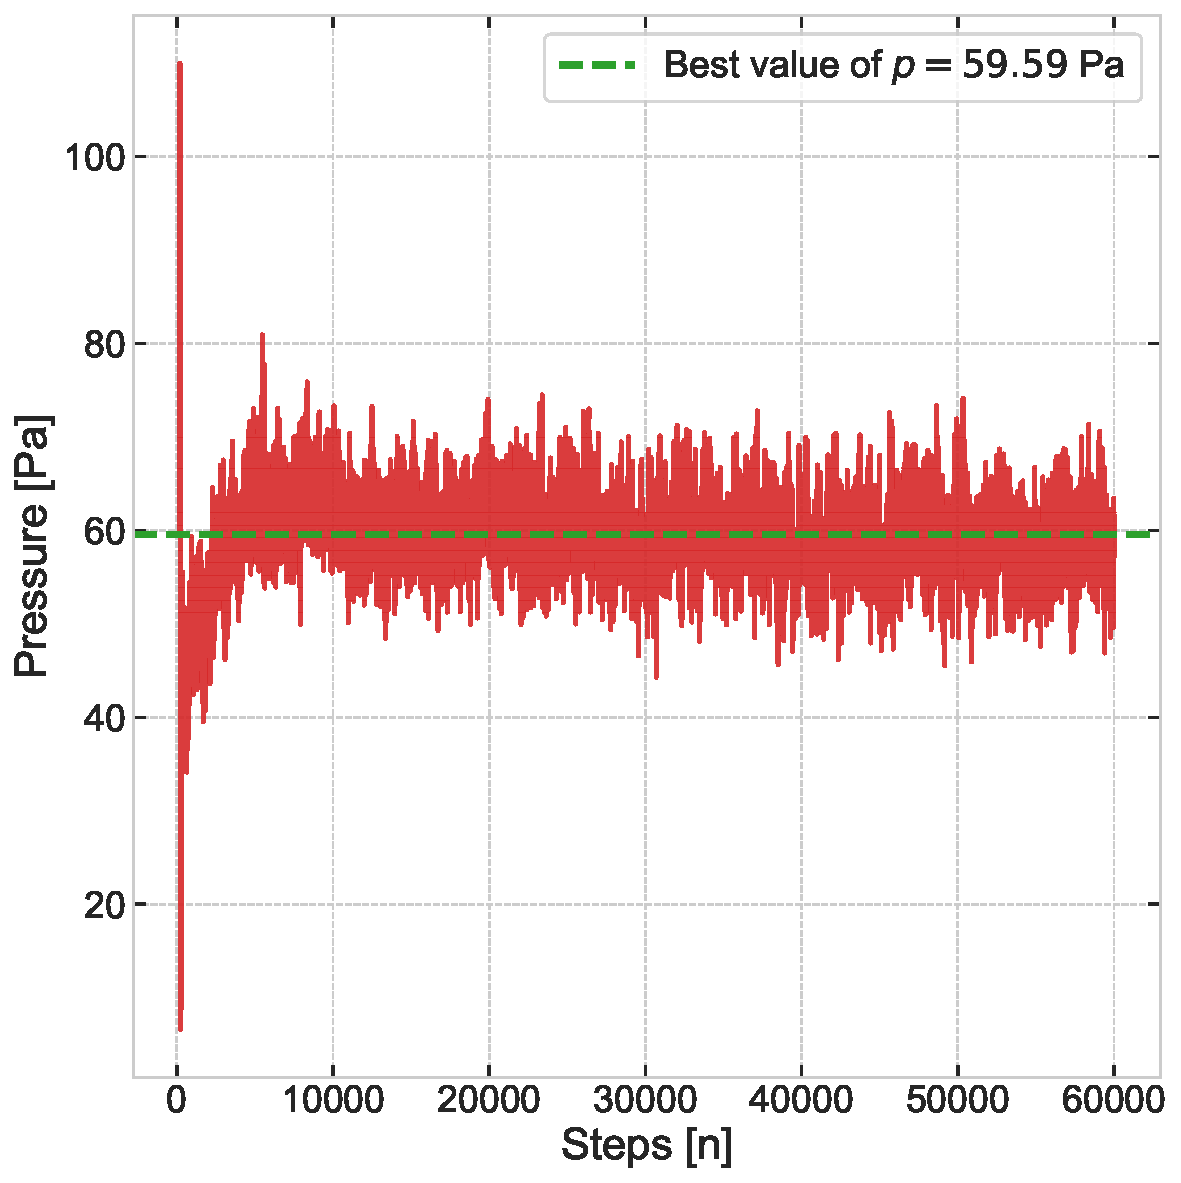
\includegraphics[width=0.45\textwidth]{{img_src/p_propagation_60000}.pdf}
    \captionof{figure}{Pressure of the system with 64 particles for $60000$ steps with dt$= 0.001$ step size.} \label{fig:13}
\end{center}
Also an exact/mean value could be given for this quantity, using the same method seen at the case of the $C_{V}$:
\begin{equation}
p
\approx
59.59\ \text{Pa}
\end{equation}
According to the ideal gas law, for this particular system ($T$, $V$, $N$) this value should be $59.941 Pa$, which is very close to my result. \par
Finally, the compressibility factor $Z$ could be given, where $Z$ by definition in our measure is
\begin{equation}
Z
=
\frac{pV}{N k_{B} T}
=
\frac{pV}{N T}
\end{equation}
I observed, that its value propagates toward the ideal gases' ($Z \to 1$) as the simulation runs longer and longer. This tendency could be seen on Fig. (\ref{fig:14}).

\begin{center}
    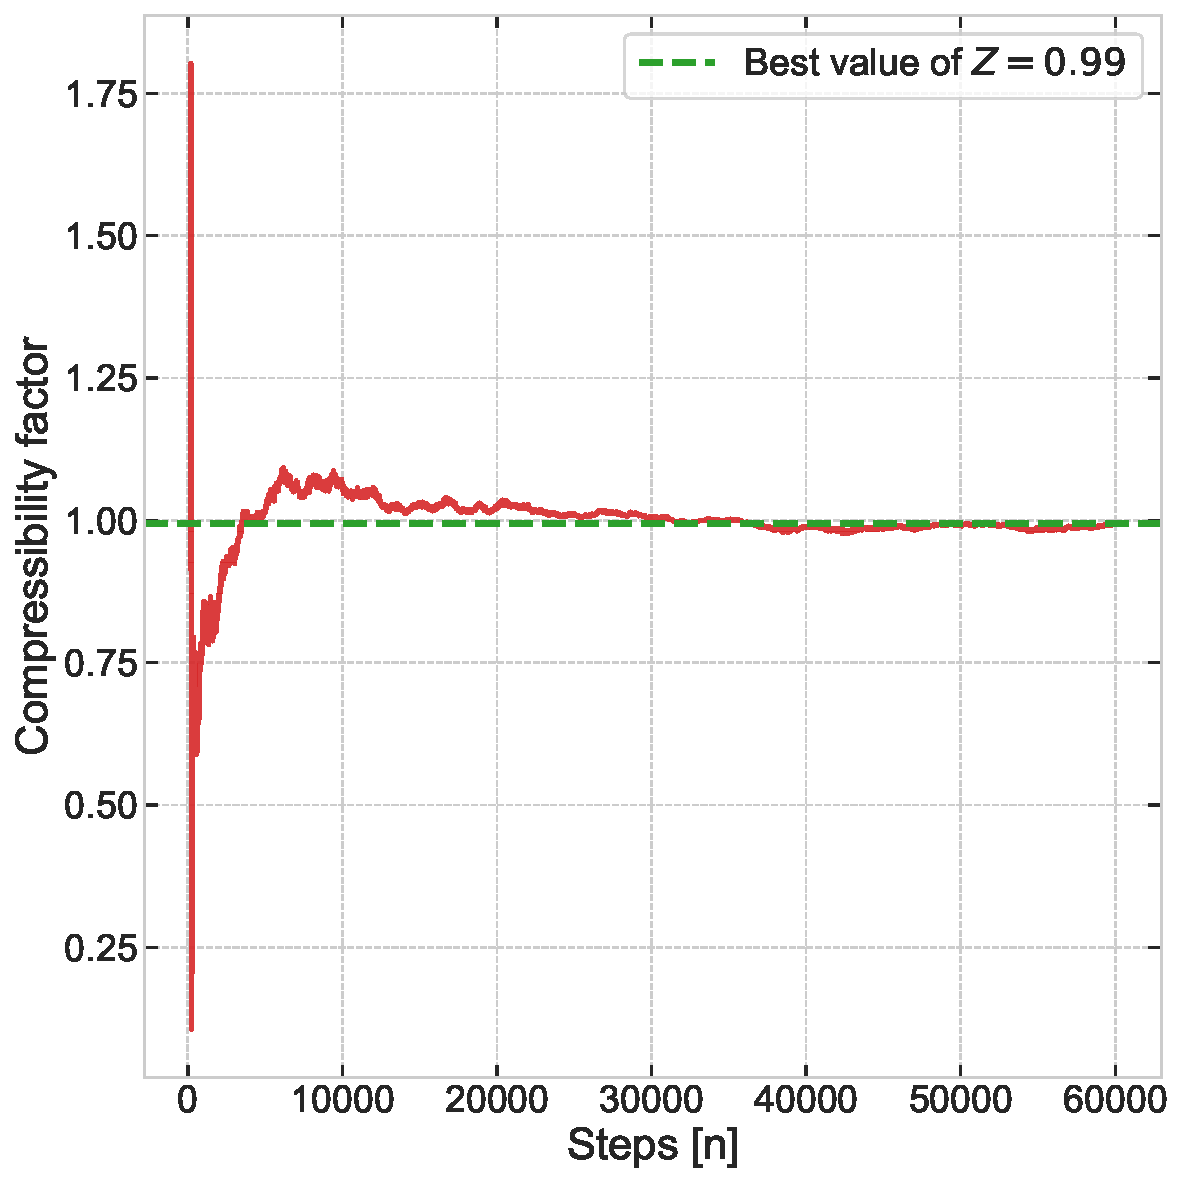
\includegraphics[width=0.45\textwidth]{{img_src/Z_propagation_60000}.pdf}
    \captionof{figure}{The changing of the compressibility factor of the system with 64 particles for $60000$ steps with dt$= 0.001$ step size.} \label{fig:14}
\end{center}

\section{Problems, limits and their solutions}
Simulations, using the Lennard-Jones potential tends to be highly unstable, when particles somehow (mostly at the start of the simulation) manage to get too close to each other. It is clear from the Lennard-Jones potential's definition that in this case the affected particles are getting inexplicably large velocities, which immediately breaks the simulation. To avoid this problem, initially I've placed the particles evenly distributed into a lattice inside the simulated volume. This made the simulation totally robust for the setting of its initial conditions. \par
The other problem I've encountered with was merely technical in its nature. To optimize runtime, I've used Python's \texttt{numba} library, to compile my functions into machine code. Without this, the simulation is pretty slow, but implementing this, it raises serious obstacles. First, \texttt{numba} treats global variables as runtime-constants and forbids the overwriting of them. Since I've treat the pair-list as a global variable it made it impossible to update it after every $10$ steps. The simulation with \texttt{numba} only works well, if the close pairs never changes at all. Thus in this for the simulation could handle large number of particles, but only with \texttt{numba} deactivated. It also makes it impossible to run the simulation with bounded boundary conditions, since the pair-list could, and will be changing for much smaller number of particles too during the running.

\section{Discussion}
Finally, I've managed to make a working molecular dynamics simulation, which raised great obstacles in my path last semester. I measured some thermodynamic quantities, which correlated with literary data as well and thus -- except some smaller problems -- I've achieved my goals declared in the short description.

\end{multicols}
